% Este archivo es parte de la memoria del proyecto fin de carrera
% de Diego Barrios Romero. Protegida bajo la licencia GFDL.
% Para más información, la licencia completa viene incluida en el
% fichero fdl-1.3.tex

% Copyright (C) 2012 Manuel López Urbina

\chapter{Montaje hardware}
\label{chap:dispositivos-hardware}

\section{Colocación de la cámara en el vehículo}

Para la obtención de la imágenes se ha elegido una pequeña cámara inalámbrica con el fin de no limitar la capacidad de movimiento del vehículo.\\

 La cámara ha sido situada en la parte delantera del vehículo en el soporte que dispone para la colocación de la misma. Destacar que se ha empleado el sistema de cámara independiente debido al estado defectuoso de la cámara original del vehículo.\\

Para la alimentación de la cámara se ha añadido una pila de 9 voltios en la parte trasera del vehículo. En la imagen \ref{fig:coche-camara-pila} se puede visualizar el conjunto vehículo, cámara y pila de alimentación montados.\\

\begin{figure}[H]
  \begin{center}
    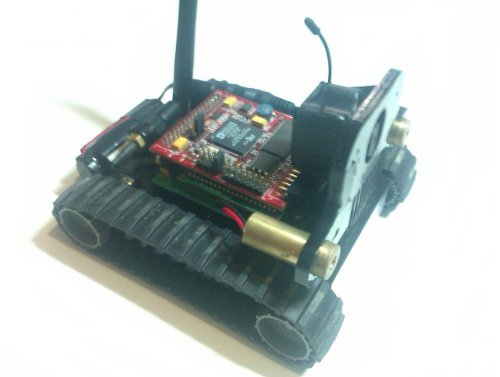
\includegraphics[scale=0.5]{coche-camara-pila.jpg}
  \end{center}
  \caption{Vehículo SRV-1 tras el montaje de la cámara.}
  \label{fig:coche-camara-pila}
\end{figure}


\section{Conexión cámara - PC}

Para conectar la cámara al ordenador, al tratarse de una cámara inalámbrica, resulta necesario utilizar un receptor. Las imágenes son trasmitidas mediante radiofrecuencia desde la cámara al sistema receptor que se encuentra conectado al PC mediante una capturadora de vídeo USB.\\

El sistema receptor de vídeo consiste en un capturador de imágenes analógico que recibe imágenes analógicas a través de radiofrecuencia. El receptor, posteriormente, a través de conectores RCA envía la imagen analógica al conversor analógico/digital convirtiendo la imagen analógica en imagen digital con una resolución de 720x576 píxeles, y que a su vez se encuentra conectado al PC mediante un cable USB, éste último dispositivo es también conocido como capturadora de vídeo.\\

El ordenador detecta la cámara como si de una webcam se tratara. El funcionamiento del sistema receptor se esquematiza en la figura \ref{esquema-sistema-receptor-video}. Indicar que el receptor de imagen analógico se alimenta con un adaptador de corriente. \\

\begin{figure}[H]
  \begin{center}
    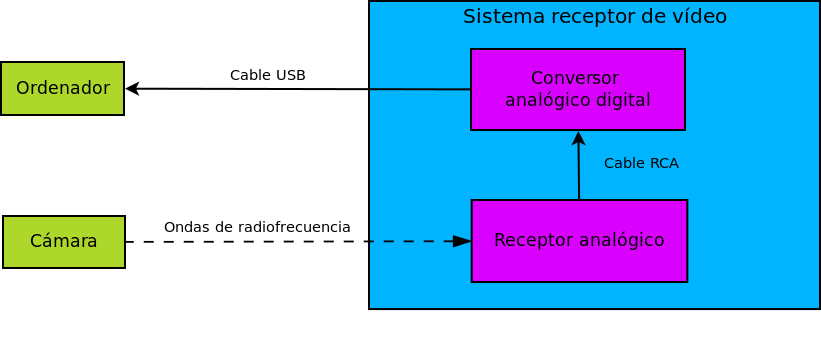
\includegraphics[scale=0.5]{esquema-sistema-receptor-video.png}
  \end{center}
  \caption{Esquema del sistema de recepción de imágenes desde la cámara al ordenador.}
  \label{esquema-sistema-receptor-video}
\end{figure}

En la figura \ref{fig:conjunto-video} se muestra una fotografía del conjunto correctamente conectado:\\

\begin{figure}[H]
  \begin{center}
    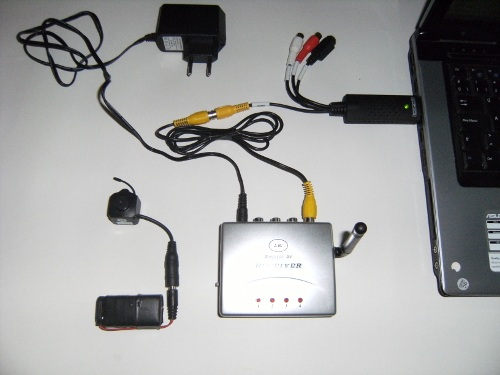
\includegraphics[scale=0.7]{conjunto-video.jpg}
  \end{center}
  \caption{Visión del sistema de recepción de imágenes montado a falta de la conexión a corriente del receptor.}
  \label{fig:conjunto-video}
\end{figure}


\section{Comunicaciones vehículo - PC}

Para establecer las comunicaciones entre el vehículo robótico y el ordenador ha sido necesario disponer de un router Wi-Fi para la creación de una infraestructura de red, de tal manera que, el vehículo SRV-1 realice automáticamente una conexión al router tras activarse el interruptor de encendido. Por otra parte, el ordenador deberá de conectarse al router como de si una red convencional se tratara. Se ha optado por este sistema debido a que presenta una mayor estabilidad que realizar una conexión directa ad hoc entre el ordenador y el vehículo.\\

En la sección \ref{sec:configuración-router} del manual de usuario se detalla el proceso de configuración del router Xavi 7868r utilizado.\\

El vehículo debe ser configurado según los valores previamente fijados en el router de tal manera que cuando el vehículo sea puesto en marcha realice una conexión de manera automática e inalámbrica con el router integrándose en la red. En el manual de usuario, sección \ref{sec:configuración-srv}, se detalla los pasos y parámetros necesarios para su correcta configuración.\\


La figura \ref{fig:com-coche-pc} de a continuación muestra un esquema de las comunicaciones entre el vehículo y el ordenador mediante el uso de un router.\\

\begin{figure}[H]
  \begin{center}
    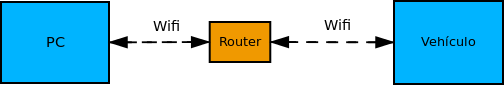
\includegraphics[scale=0.8]{comunicacion-coche-robot.png}
  \end{center}
  \caption{Comunicaciones vía Wi-Fi entre el ordenador y el vehículo robótico mediante un router.}
  \label{fig:com-coche-pc}
\end{figure}


\begin{figure}[H]
  \begin{center}
    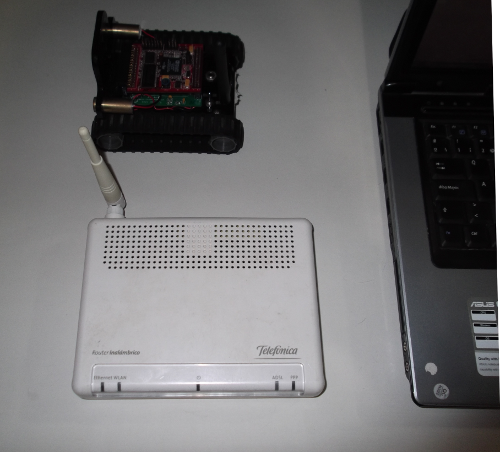
\includegraphics[scale=0.6]{sistema-comunicaciones-coche-pc.png}
  \end{center}
  \caption{Vista del sistema de comunicaciones entre el vehículo y el ordenador.}
  \label{fig:conjunto-video}
\end{figure}

